\subsection{Approssimazione di funzioni e di dati}

\subsubsection{Interpolazione Lagrangiana e Composita Lineare}

\begin{flushleft}
	\textbf{\underline{Esercizio 1}}
\end{flushleft}
Si valuti il problema dell'approssimazione della funzione di Runge:
\begin{equation*}
	f\left(x\right) = \dfrac{1}{1+x^{2}}
\end{equation*}
Mediante un'interpolazione polinomiale di Lagrange nell'intervallo $I = \left[-5, 5\right]$. Si costruiscano i polinomi interpolanti $\prod_{n}f$ e dell'errore $E_{n}f\left(x\right) = \left|f\left(x\right) - \prod_{n}f\left(x\right)\right|$ e si calcoli $\left|\left|E_{n}f\right|\right|_{\infty}$:
\begin{equation*}
	\left|\left|E_{n}f\right|\right|_{\infty} = \underset{x \in \left[-5, 5\right]}{\max} \left|f\left(x\right) - \prod_{n}f\left(x\right)\right|
\end{equation*}

\highspace
Si costruisce il polinomio interpolante $\prod_{n}f\left(x\right)$ di grado $n = 5$, $10$ della funzione $f$ considerando nodi equispaziati sull'intervallo $I$. Per ciascun valore di $n$ si vuole rappresentare graficamente $\prod_{n}f\left(x\right)$ e l'errore $E_{n}f\left(x\right) = \left|f\left(x\right) - \prod_{n}f\left(x\right)\right|$.
\begin{enumerate}
	\item Si definisce la funzione di Runge.
	\lstinputlisting[language=MATLAB]{code/approssimazione-di-funzioni-e-di-dati/interpolazione_1.m}
	
	\item Si memorizzano gli estremi dell'intervallo $I$ nelle variabili $a,b$ e il vettore contenente le ascisse degli $n+1$ nodi equispaziati.
	\lstinputlisting[language=MATLAB]{code/approssimazione-di-funzioni-e-di-dati/interpolazione_2.m}
	
	\item Si procede valutando la funzione in corrispondenza dei nodi.
	\lstinputlisting[language=MATLAB]{code/approssimazione-di-funzioni-e-di-dati/interpolazione_3.m}
	
	\item Si realizza il polinomio interpolante utilizzando le funzioni \texttt{polyfit} e \texttt{polyval}.
	\lstinputlisting[language=MATLAB]{code/approssimazione-di-funzioni-e-di-dati/interpolazione_4.m}
	
	\item Si visualizza il grafico della funzione e del polinomio interpolante $\prod_{n}f$ nell'intervallo $I$.
	\lstinputlisting[language=MATLAB]{code/approssimazione-di-funzioni-e-di-dati/interpolazione_5.m}
	\newpage
	\begin{figure}[!htp]
		\centering
		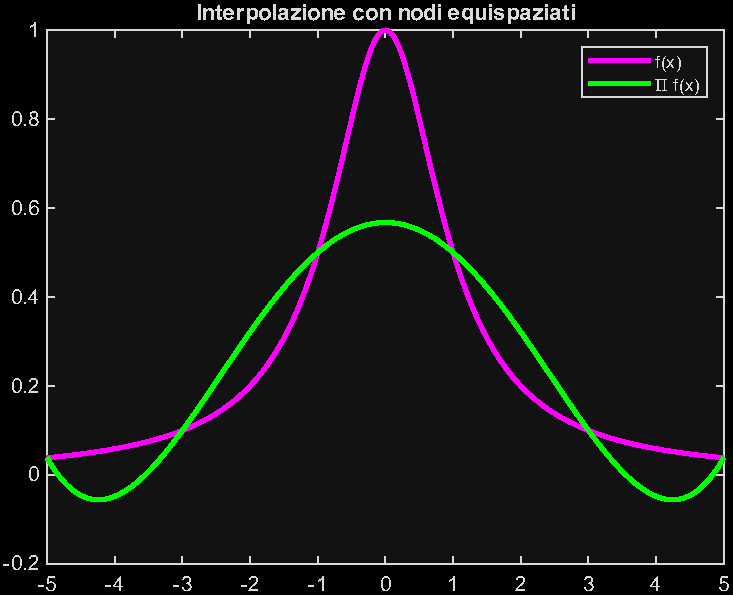
\includegraphics[width=.7\textwidth]{img/interpolazione-1.pdf}
	\end{figure}
	
	\item Infine si studia l'andamento dell'errore $E_{n}f\left(x\right)$ e lo si rappresenta graficamente.
	\lstinputlisting[language=MATLAB]{code/approssimazione-di-funzioni-e-di-dati/interpolazione_6.m}
	\begin{figure}[!htp]
		\centering
		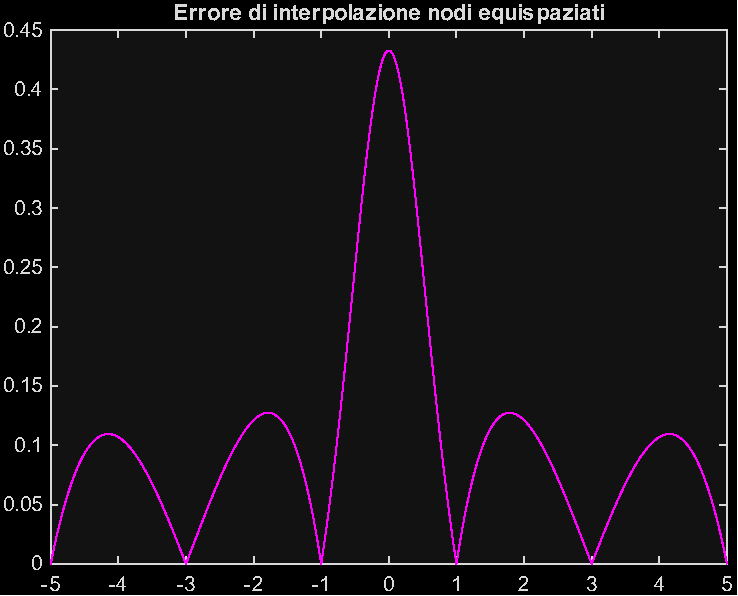
\includegraphics[width=.7\textwidth]{img/interpolazione-2.pdf}
	\end{figure}
\end{enumerate}

\newpage

\begin{flushleft}
	\textbf{\underline{Esercizio 2}}
\end{flushleft}
Nella tabella sotto riportata vengono elencati i risultati di un esperimento eseguito per individuare il legame tra lo \emph{sforzo} $\sigma$ e la relativa \emph{deformazione} $\varepsilon$ di un campione di un tessuto biologico.
\begin{table}[!htp]
	\centering
	\begin{tabular}{@{} c c c @{}}
		\toprule
		test & $\sigma$ [MPa] & $\varepsilon$ [cm/cm] \\
		\midrule
		1 & 0.00 & 0.00 \\
		2 & 0.06 & 0.08 \\
		3 & 0.14 & 0.14 \\
		4 & 0.25 & 0.20 \\
		5 & 0.31 & 0.23 \\
		6 & 0.47 & 0.25 \\
		7 & 0.60 & 0.28 \\
		8 & 0.70 & 0.29 \\
		\bottomrule
	\end{tabular}
\end{table}

\noindent
A partire da questi dati si vuole stimare, utilizzando opportune tecniche di interpolazione, la deformazione $\varepsilon$ del tessuto in corrispondenza dei valori di sforzo per cui non si ha a disposizione un dato sperimentale. A tal fine, si considerino le seguenti funzioni interpolanti:
\begin{itemize}
	\item Interpolazione polinomiale di Lagrange (\texttt{polyfit} e \texttt{polyval});
	\item Interpolazione polinomiale composita lineare (\texttt{interp1});
\end{itemize}
In particolare, a partire dal codice assegnato si vuole:
\begin{enumerate}
	\item Rappresentare graficamente le singole funzioni interpolanti a confronto con i dati sperimentali;

	\item Confrontare in un unico grafico i dati sperimentali con tutte le funzioni interpolanti;
	
	\item Valutare, per ogni interpolante, la deformazione $\varepsilon$ in corrispondenza di $\sigma = 0.40$ MPa e $\sigma = 0.75$ MPa;
	
	\item Commentare i risultati ottenuti.
\end{enumerate}

\newpage

\noindent
La soluzione:
\begin{enumerate}
	\item Si definiscono in MATLAB i vettori componenti i dati sperimentali \texttt{sigma} (per lo sforzo $\sigma$) ed \texttt{epsilon} (per la deformazione $\varepsilon$).
	\lstinputlisting[language=MATLAB]{code/approssimazione-di-funzioni-e-di-dati/interpolazione_7.m}
	
	\item In figura viene riportato il grafico dei dati sperimentali, ottenuto con le seguenti istruzioni.
	\lstinputlisting[language=MATLAB]{code/approssimazione-di-funzioni-e-di-dati/interpolazione_8.m}
	\begin{figure}[!htp]
		\centering
		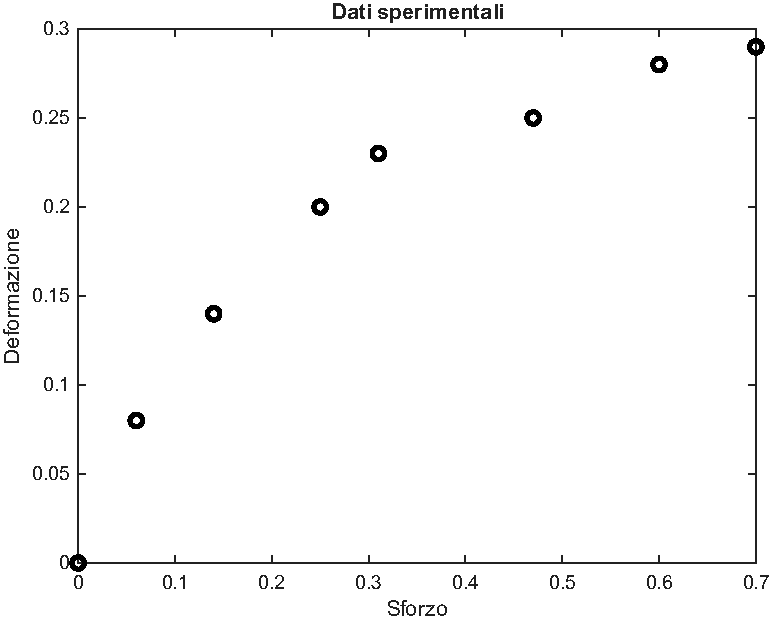
\includegraphics[width=.7\textwidth]{img/interpolazione-3.pdf}
	\end{figure}
	
	\item L'\emph{interpolazione polinomiale di Lagrange} viene realizzata mediante le funzioni MATLAB \texttt{polyfit} e \texttt{polyval}. Si ricorda che il numero di punti corrispondenti ai dati sperimentali determina (per definizione) il grado del polinomio di Lagrange, pari al numero di punti meno uno. Per disegnare il polinomio interpolatore di Lagrange si eseguono i seguenti comandi:
	\lstinputlisting[language=MATLAB]{code/approssimazione-di-funzioni-e-di-dati/interpolazione_9.m}
	\newpage
	\begin{figure}[!htp]
		\centering
		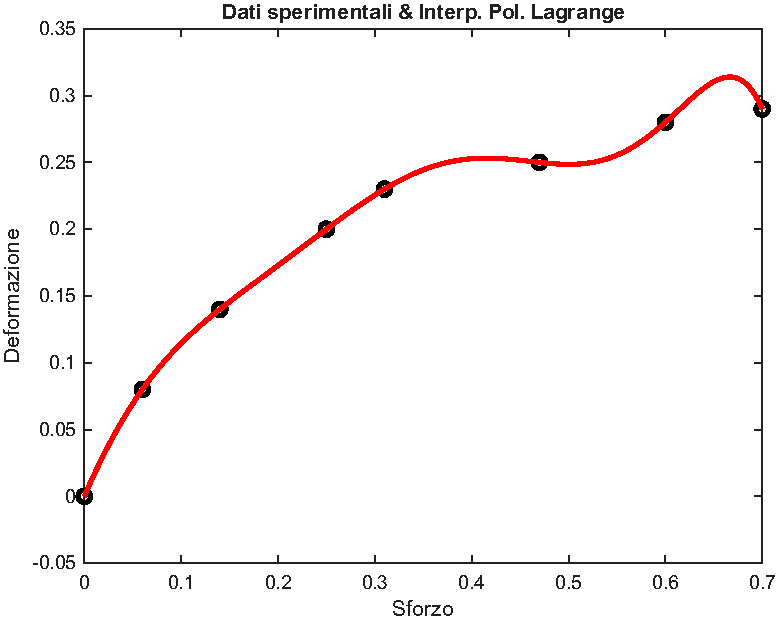
\includegraphics[width=.7\textwidth]{img/interpolazione-4.pdf}
	\end{figure}
\end{enumerate}